\documentclass[a4paper,11pt,final]{report}
\usepackage[utf8]{inputenc} % Prendre en compte les caractères accentués
\usepackage[francais]{babel} % Prendre en compte les particularités de la typographie française.
\usepackage{geometry}         % marges
\usepackage{graphicx}         % images
\usepackage{setspace}
\usepackage[french]{varioref}
\usepackage{titlesec}  %titlespacing
\usepackage{caption}

\titlespacing{\chapter}{0pt}{*-5}{*5}
\titlespacing{\section}{0pt}{*2}{*2}
\titleformat{\chapter}[hang]{\bf\huge}{\thechapter}{2pc}{}
%\titleformat{\chapter}[hang]{\bf\huge}{\thechapter}{14pt}{\LARGE}
\renewcommand{\baselinestretch}{1.2}
\setlength{\parskip}{1.5ex plus .4ex minus .4ex}
\setlength{\parindent}{15pt} 
%\setlength{\topmargin}{-35pt}
%\setlength{\textheight}{600pt}


\title{\textbf{Manuel d'utilisation}\\E-Formulaire}
\author{}
\date{}
\begin{document}

\maketitle
\setcounter{page}{2}
\tableofcontents 
%Se mettre au niveau d'un non informaticien
%Expliquer les enchainements de fenêtre, erreurs
%FAQ
\chapter{Généralités}
\section{But de l'application}
Uniforms a pour but de fournir une plateforme de gestion de formulaires. C'est-à-dire, proposer des fonctionnalités de création et de soumission de formulaires ainsi que la possibilité de répondre à ces derniers et de consulter les réponses par le créateur du formulaire.

\section{Public visé}
Ce manuel est destiné aux personnes désirant créer un formulaire, le soumettre à une ou plusieurs personnes et consulter les réponses faites par les destinataires, mais aussi aux personnes répondant aux formulaires envoyés par l'intermédiaire de la plateforme uniforms.

\section{Installation}

\section{Support technique}

\chapter{Fenêtre principale}
\section{Authentification}
La première page affichée est celle de l'authentification, que l'on peut voir figure~\ref{authentificationChoix}, elle en propose deux types : CAS (pour les utilisateurs disposants d'un identificant CAS commençant par les initiales du nom et prénom puis du numéro étudiant) ou autres utilisateurs.\\
%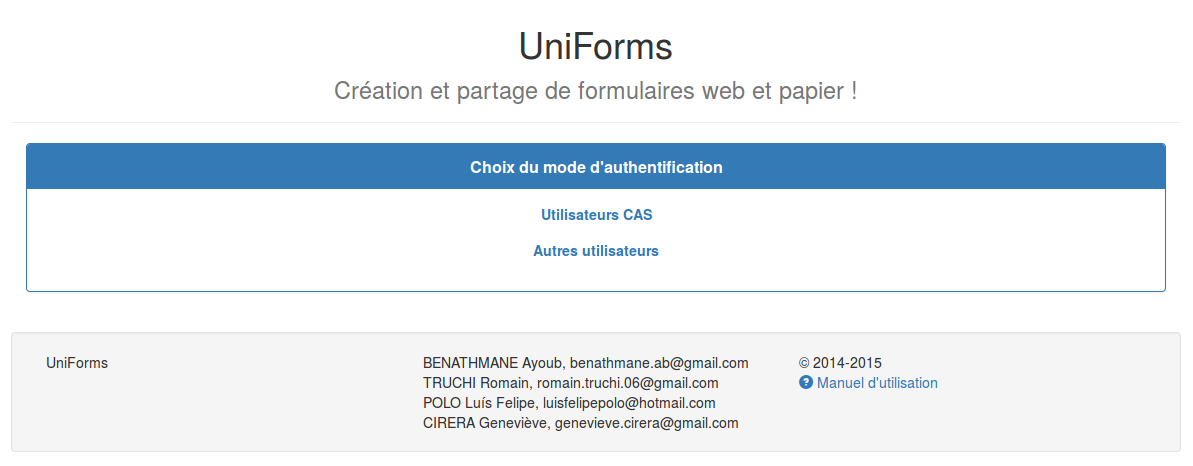
\includegraphics[width=.7\paperwidth]{images/authentification.png}\label{fig:ArgSimple}
\noindent\begin{minipage}{\linewidth}% to keep image and caption on one page
\makebox[\linewidth]{%        to center the image
  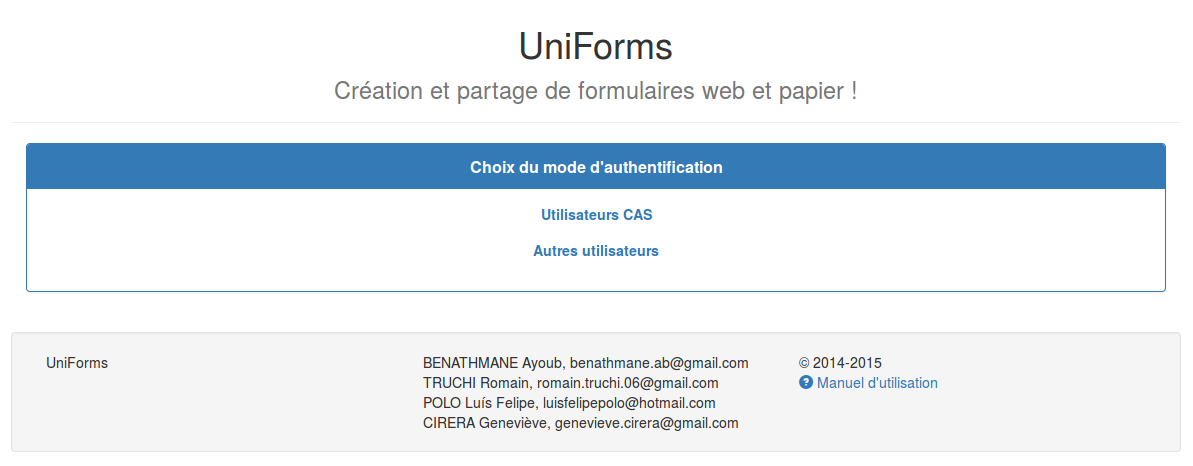
\includegraphics [width=150mm]{images/authentification.png}}
\captionof{figure}{Page de choix d'authentification}\label{authentificationChoix}
\end{minipage}

Pour accéder à la page d'authentification, il suffit de cliquer sur ``Utilisateurs CAS'' ou ``Autres utilisateurs''
\subsection{Utilisateur CAS}
Une fois choisi l'authentification CAS, la page figure~\ref{authentificationCAS} s'affiche.\\
Dans le champs ``Identification'', mettre votre identifiant (ex : dj209832, pour Jean Dupont ayant pour numéro étudiant 209832).\\
Entrer le mot de passe puis cliquer sur ``SE CONNECTER''. Si l'authentification échoue, une alerte ``Mauvais identifiant / mot de passe'' apparaitra pour vous en informer. Si elle réussit, la page d'accueil, figure~\ref{pageAccueil}, s'affichera. 

\noindent\begin{minipage}{\linewidth}% to keep image and caption on one page
\makebox[\linewidth]{%        to center the image
  
\includegraphics [width=150mm]{images/authCAS.png}}
\captionof{figure}{Authentification CAS}\label{authentificationCAS}
\end{minipage}
\subsection{Autres utilisateurs}

\section{Page d'accueil}
Après authentification, la page figure~\ref{pageAccueil} s'affiche. On peut noter trois zones principales, une barre d'option, une zone de formulaires créés, une zone de formulaires à répondre.\\
\noindent\begin{minipage}{\linewidth}% to keep image and caption on one page
\makebox[\linewidth]{%        to center the image
  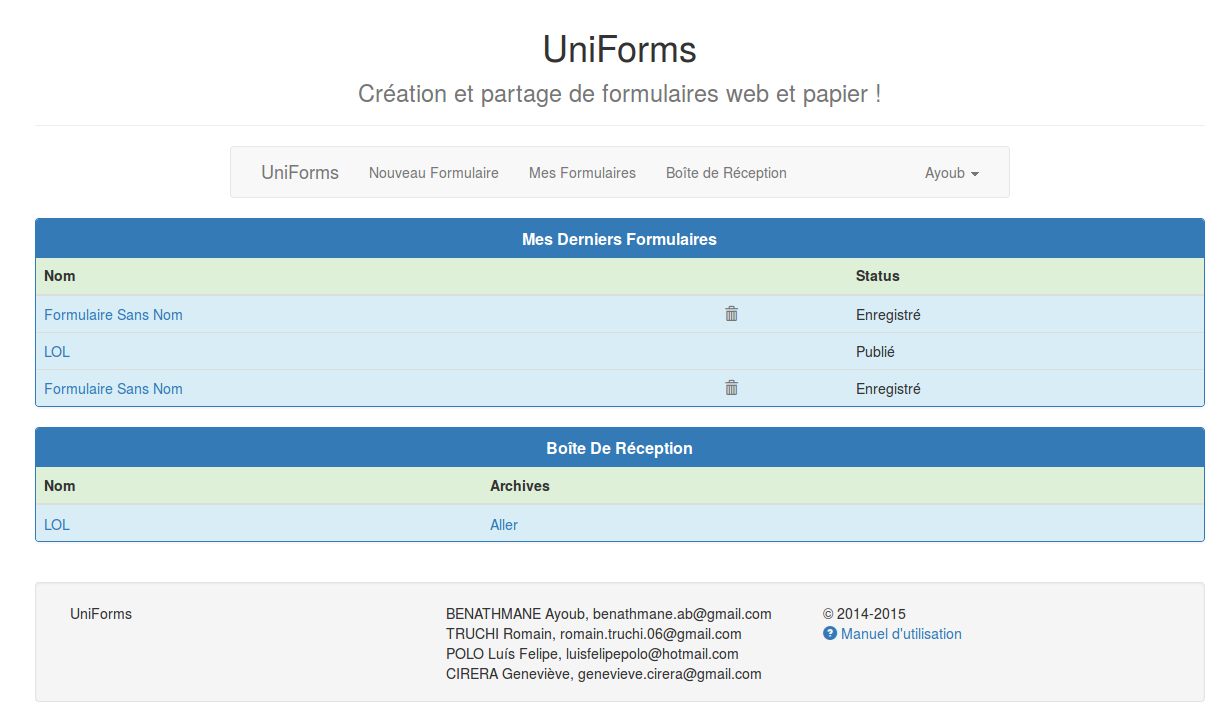
\includegraphics [width=190mm]{images/pageAccueil.png}}
\captionof{figure}{Page d'accueil}\label{pageAccueil}
\end{minipage}

\subsection{La barre d'options}\label{sec:barreOption}
La barre d'options figure~\ref{barreOptions} propose divers boutons : ``Uniforms'', ``Créer un formulaire'', ``Mes Archives'' et ``Ayoub''. Les actions au clique de ces boutons sont les suivantes :
\begin{description}
	\item [Uniform] : Retour à la page d'accueil
	\item [Créer un formulaire] : Redirection vers la page de création d'un nouveau formulaire
	\item [Mes archives] : Redirection vers les formulaires archivés
	\item [Ayoub] : Identifiant de la personne dont la session est ouverte, au clique l'option ``Logout'' s'affiche pour la déconnection.
\end{description}

\noindent\begin{minipage}{\linewidth}% to keep image and caption on one page
\makebox[\linewidth]{%        to center the image
  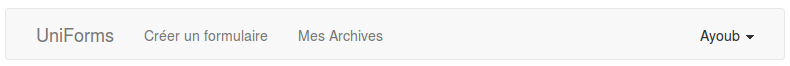
\includegraphics [width=140mm]{images/barreOptionsAccueil.png}}
\captionof{figure}{Barre d'options}\label{barreOptions}
\end{minipage}

\subsection{Zone de formulaires créés}
La zone de formulaires créés liste l'ensemble des formulaires créés par l'utilisateur courant, les validés et non validés, figure~\ref{zoneFormCree}.\\
Un formulaire validé ou non peut être supprimé en cliquant sur la corbeille de la colonne ``Supprimer'' correspondante.

\noindent\begin{minipage}{\linewidth}% to keep image and caption on one page
\makebox[\linewidth]{%        to center the image
  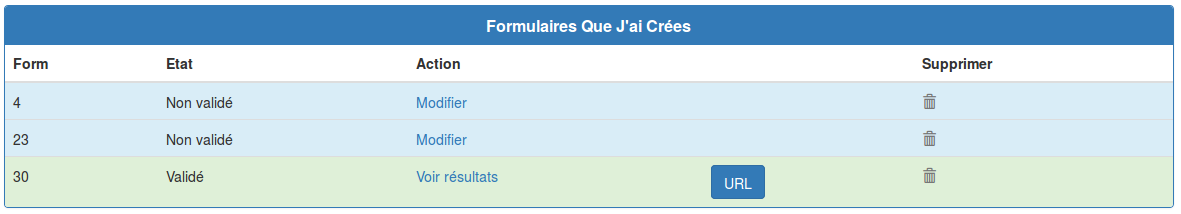
\includegraphics [width=140mm]{images/zoneFormulairesCreesAccueil.png}}
\captionof{figure}{Liste des formulaires créés}\label{zoneFormCree}
\end{minipage}

\subsubsection{Les formulaires validés}
Les formulaires validés ne peuvent plus être modifié, ils ont été envoyés aux destinataires. Les seules actions possibles sur ces formulaires sont ``Voir résultats'' qui montre les réponses du formulaire qui ont déjà été faites par les destinataires et ``Supprimer''. On peut également obtenir l'url en cliquant sur le bouton ``URL'' de ce formulaire afin de l'envoyer par mail à un destinataire.

\noindent\begin{minipage}{\linewidth}% to keep image and caption on one page
\makebox[\linewidth]{%        to center the image
  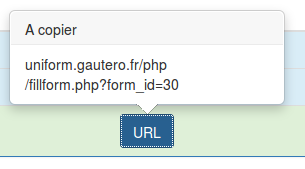
\includegraphics [width=40mm]{images/urlForm.png}}
\captionof{figure}{URL d'un formulaire validé}\label{urlForm}
\end{minipage}

\subsubsection{Les formulaires non validés}
Les formulaires non validés n'ont pas encore été envoyés aux destinataires, ils peuvent donc être modifiés en cliquant sur le lien ``Modifier'' de la ligne du formulaire souhaité. Cette action mènera à la page ...???

\subsection{Zone de formulaires reçus}
Dans cette zone figure~\ref{zoneFormRecu} est listé l'ensemble des formulaires dont l'utilisateur courant est destinataire, c'est-à-dire ceux pour lesquels il doit répondre.\\
La liste des réponses en cours sont en bleus. Certains formulaires autorisent plusieurs réponses, c'est pourquoi on verra les lignes ``Réponse\string:0'', ``Réponse\string:1'', ``Réponse\string:2'' figure~\ref{zoneFormRecu} lorsque celles-ci sont initiés mais non validées.\\
Lorsque toutes les réponses autorisées ne sont pas initiées et/ou envoyées, le nombre restant est indiqué en vert, par exemple le formulaire 6 figure~\ref{zoneFormRecu} autorise 2 réponses en plus de celle initiée ``Réponse\string:0'' de la ligne juste en dessous.\\
Une fois toutes les réponses envoyés, seule la ligne du formulaire est présente, par exemple le formulaire 5 de la figure figure~\ref{zoneFormRecu}.\\

Les liens ``Modifier'' permettent la modification d'une réponse déjà commencée. Le lien ``Nouvelle réponse'' permet de commencer une réponse à un formulaire.

\noindent\begin{minipage}{\linewidth}% to keep image and caption on one page
\makebox[\linewidth]{%        to center the image
  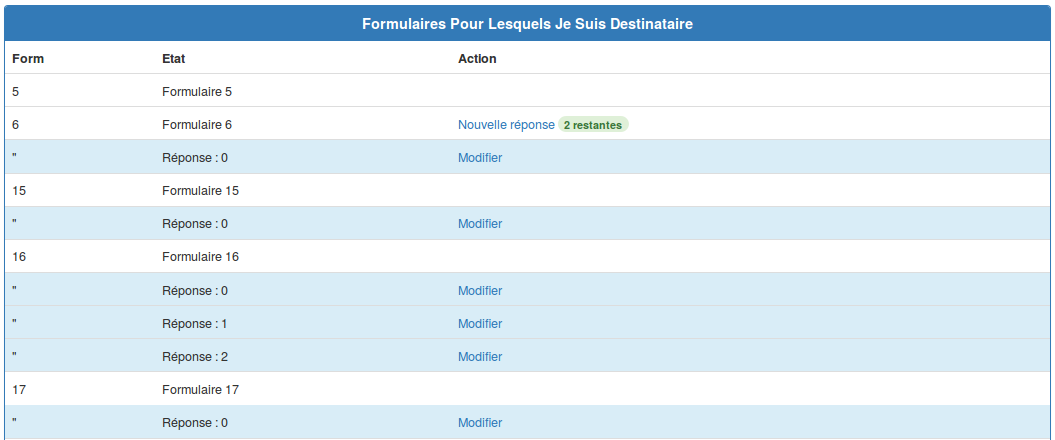
\includegraphics [width=150mm]{images/zoneDestinataire.png}}
\captionof{figure}{Zone de formualaires reçus}\label{zoneFormRecu}
\end{minipage}

\chapter{Création}
\section{Créer un formulaire}\label{CreerFormulaire}
Pour créer un formulaire, la première étape est de cliquer sur le bouton ``Créer un formulaire'' de la barre d'options, voir figure~\ref{barreOptions}. Ensuite la page de création, figure~\ref{pageCreation}, s'affiche.\\
On peut distinguer plusieurs zones. On retrouve tout d'abord la barre d'option vu section~\ref{sec:barreOption}, puis une zone de ``Paramètre'', une zone de ``Destinataires'', une zone avec une page quadriée puis sur les cotés, une zone de ``Groupe'' à gauche et une zone d'éléments à droite.\\
Tout en bas de cette page, deux boutons ``Enregistrer'' et ``Valider'', permettant respectivement d'enregistrer un formulaire (afin de pouvoir le modifier par la suite) et de valider un formulaire, ce dernier sera alors envoyé aux destinataires, aucune modification ne sera permise.

\noindent\begin{minipage}{\linewidth}% to keep image and caption on one page
\makebox[\linewidth]{%        to center the image
  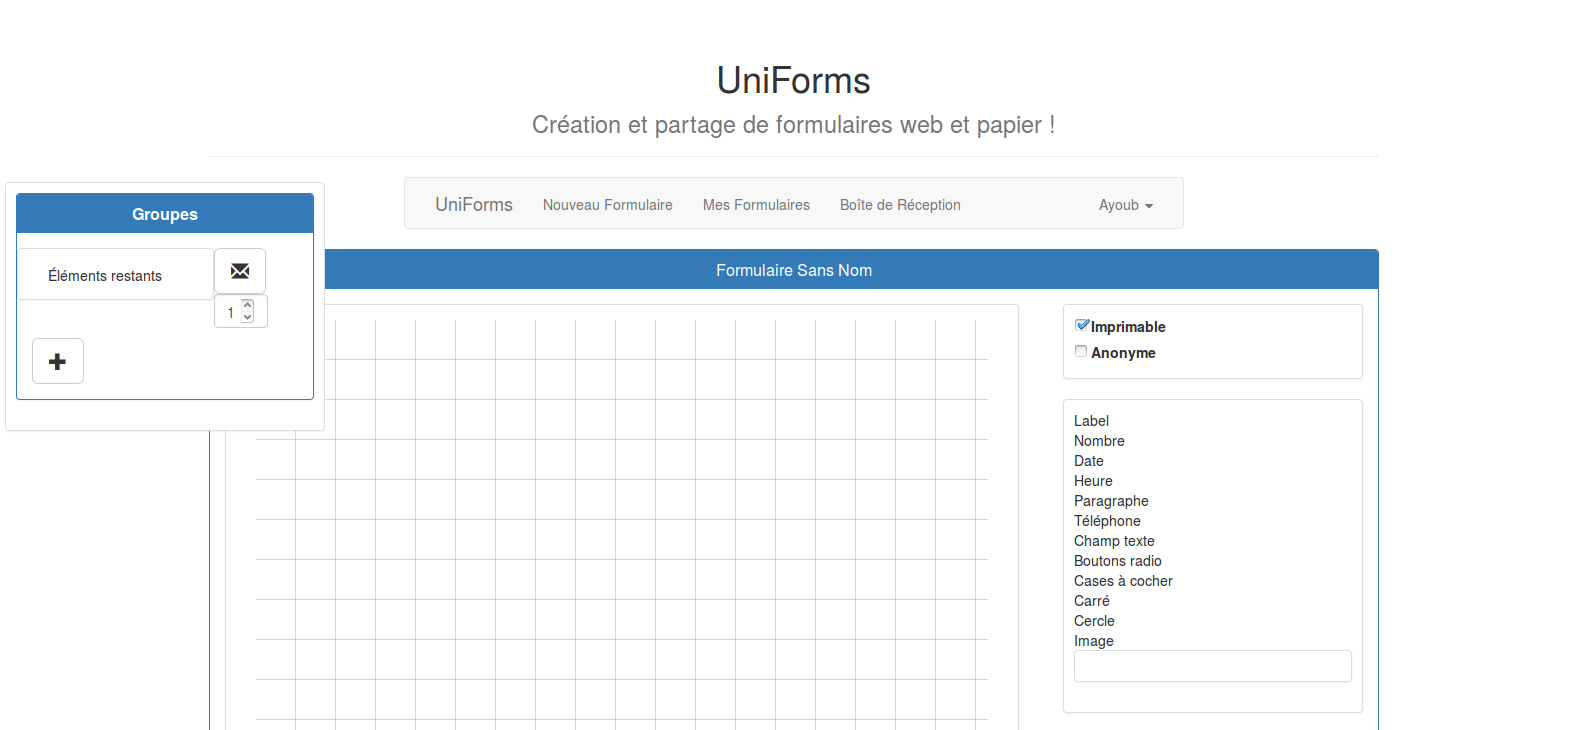
\includegraphics [width=150mm]{images/pageCreation.png}}
\captionof{figure}{Page de création de formulaire}\label{pageCreation}
\end{minipage}

\subsection{Zone de ``Paramètres''}
Trois champs sont paramètrables, figure~\ref{parametreCreation} :
\begin{description}
	\item [Imprimable] : à cocher si vous souhaitez imprimer le formulaire
	\item [Anonyme] : à cocher si vous ne souhaitez pas définir de destinataire en particulier. Ce formulaire sera donc en accès libre à toutes les personnes disposants de son lien url.
	\item [Nombre de réponses max] : Vous pouvez définir le nombre de réponse possible pour le formulaire. Si vous mettez ``3'', chaque destinataire pourra répondre trois fois à ce même formulaire. Si vous souhaitez que le nombre de réponses soit infini, mettez ``0''.
\end{description}

\noindent\begin{minipage}{\linewidth}% to keep image and caption on one page
\makebox[\linewidth]{%        to center the image
  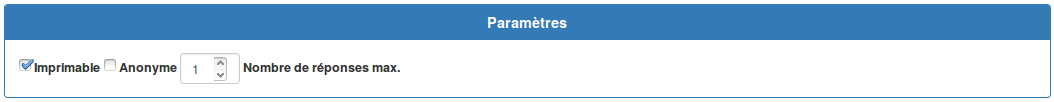
\includegraphics [width=150mm]{images/parametresCreation.png}}
\captionof{figure}{Paramètres de création de formulaire}\label{parametreCreation}
\end{minipage}

\subsection{Zone de ``Destinataires''}
Pour l'instant je la fais pas, ça risque fortement de changer.

\subsection{Zone de ``Groupe''}
Ici, je sais pas si au final, ça fonctionnera, dans le doute...

\subsection{Éléments}
Onze éléments sont disponibles, figure~\ref{elements}, pour les utiliser il suffit de les drag'n'dropper avec la souris sur la page quadriée. Vous trouverez en annexe, le descriptif de chaque élément.

\noindent\begin{minipage}{\linewidth}% to keep image and caption on one page
\makebox[\linewidth]{%        to center the image
  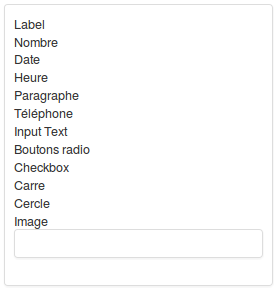
\includegraphics [width=60mm]{images/elements.png}}
\captionof{figure}{Éléments disponibles pour la création}\label{elements}
\end{minipage}

%\begin{description}
%	\item [Label] : Pour ajouter du texte, le texte doit être rempli par la zone ``Value'' qui s'affichera dès le drop du label.
%	\item [Nombre] : Champs d'entrée d'un nombre, il peut être paramétré par une valeur minimale et une valeur maximale.
%	\item [Date] : Champs d'entrée d'une date
%	\item [Heure] : Champs d'entrée d'une heure
%	\item [Paragraphe] : Champs de paragraphe
%	\item [Téléphone] : Champs d'entrée d'un numéro de téléphone
%	\item [Input Text] : Champs d'entrée de texte
%	\item [Boutons radios] : 
%	\item [Checkbox] :
%	\item [Carre] :
%	\item [Cercle] :
%	\item [Image] :
%\end{description}
\subsubsection{Ajouter un élément}
Pour ajouter un élément, le placer par drag'n'drop\footnote{Drag'n'drop : maintenir appuyer sur l'élément et déplacer la souris jusqu'à la zone choisie, relacher la pression} sur la zone quadriée.\\ 
L'élément est ensuite paramétrable par une série de champs s'affichant en dessous de la liste des éléments personnels à chaque type d'élément.
Si un élément est placé à l'extérieur de la zone autorisé, il reviendra à sa place d'origine.

\subsubsection{Modifier un élément}
Pour modifier un élément, cliquer sur celui-ci, il s'encadre alors en rouge et les champs de paramétrage s'affiche à droite. Modifier les valeurs souhaitées. La taille hauteur et largeur peuvent également être modifiées par la souris. Par survol de la souris, une flèche apparait en bas à droite de l'élément (s'il est possible de le redimensionner), elle permet le redimensionnement de l'élément.\\
Vous pouvez également déplacer l'élément par un simple drag'n'drop à l'intérieur de la zone quadriée.

\subsubsection{Supprimer un élément}
Pour supprimer un élément, il suffit de sélectionner l'élément, il doit apparaitre encadré en rouge, puis de presser la touche ``Del'' ou ``Suppr''.

\subsection{Page quadriée}
La page quadriée est la zone du formulaire, les éléments y sont placés. La hauteur et la largeur de cette zone est celle d'une page A4, la délimitation entre deux pages différente est marquée par trait noir horizontal.\\
Lors de l'ajout d'élément, si un élément est placé bas dans la page, la zone s'aggrandit automatiquement de la hauteur d'une page A4. 

\section{Modifier un formulaire}
Pour modifier un formulaire, il faut tout d'abord cliquer sur ``Modifier'' du formulaire que l'on souhaite modifier sur la page d'accueil, ce qui ouvrira la page de création de formulaire vue section~\ref{CreerFormulaire}. Cette page est remplie par les éléments, destinataires et paramètres enregistrés précédemment. Vous pouvez alors modifier ce que vous souhaitez, le ré-enregistrer ou le valider.


\section{Consulter les réponses d'un formulaire}

\chapter{Répondre}
\section{Répondre à un formulaire}

\section{Modifier ma réponse}


\chapter{FAQ}
\section{Où sont les formulaires auxquels je peux répondre ?}
\section{Puis-je modifier la réponse d'un formulaire validée ?}

\chapter{Annexe}
\section{Description des éléments}
\subsection{Label}
Si vous souhaitez placer du texte dans le formulaire, mettez un label, puis remplissez la valeur ``Value'' des paramètres par le texte désiré.
\subsection{Nombre}
Si vous souhaitez mettre un champs d'entrée que le destinataire devra remplir par un nombre, mettez un champs nombre. Vous pouvez paramétrer le nombre minimum et maximum que les destinataires seront autorisés à remplir.
\subsection{Date}
Pour un champs de date.
\subsection{Heure}
Pour un champs de heure.
\subsection{Paragraphe}
Si vous souhaitez proposer aux destinataires un champs plus large pour écrire un paragraphe.
\subsection{Input Text}
Si vous souhaitez proposer aux destinataires un champs de texte court.
\subsection{Boutons radios}
Si vous souhaitez proposer aux destinataires plusieurs choix mais qu'il ne puisse en selectionner qu'un, mettez des boutons radios. Après son placement sur la page quadrillée, un bouton ``+'' apparaitra dans la zone de paramétrage des éléments. Cliquez sur ``+'' pour pouvoir ajouter des valeurs. Cliquez sur ``-'' pour en éliminer.
\subsection{Checkbox}
Les checkbox fonctionne comme les boutons radios sauf que les destinataires pourront sélectionner plusieurs réponses au lieu d'une unique.
\subsection{Carré}
Si vous souhaitez placer un carré redimensionnable par la suite en rectangle de n'importe quelle taille.
\subsection{Cercle}
Si vous souhaitez placer un cercle redimensionnable par la suite en ovale de n'importe quelle taille.
\subsection{Image}
Si vous souhaitez insérer une image dans le formulaire, drag'n'droppez ``Image'' puis cliquez sur ``Browse'', sélectionnez enfin l'image voulu. Elle s'affichera dans le formulaire.

\end{document}
